\section{The \famsec Framework}
    \begin{figure}[tbp]
        \centering
        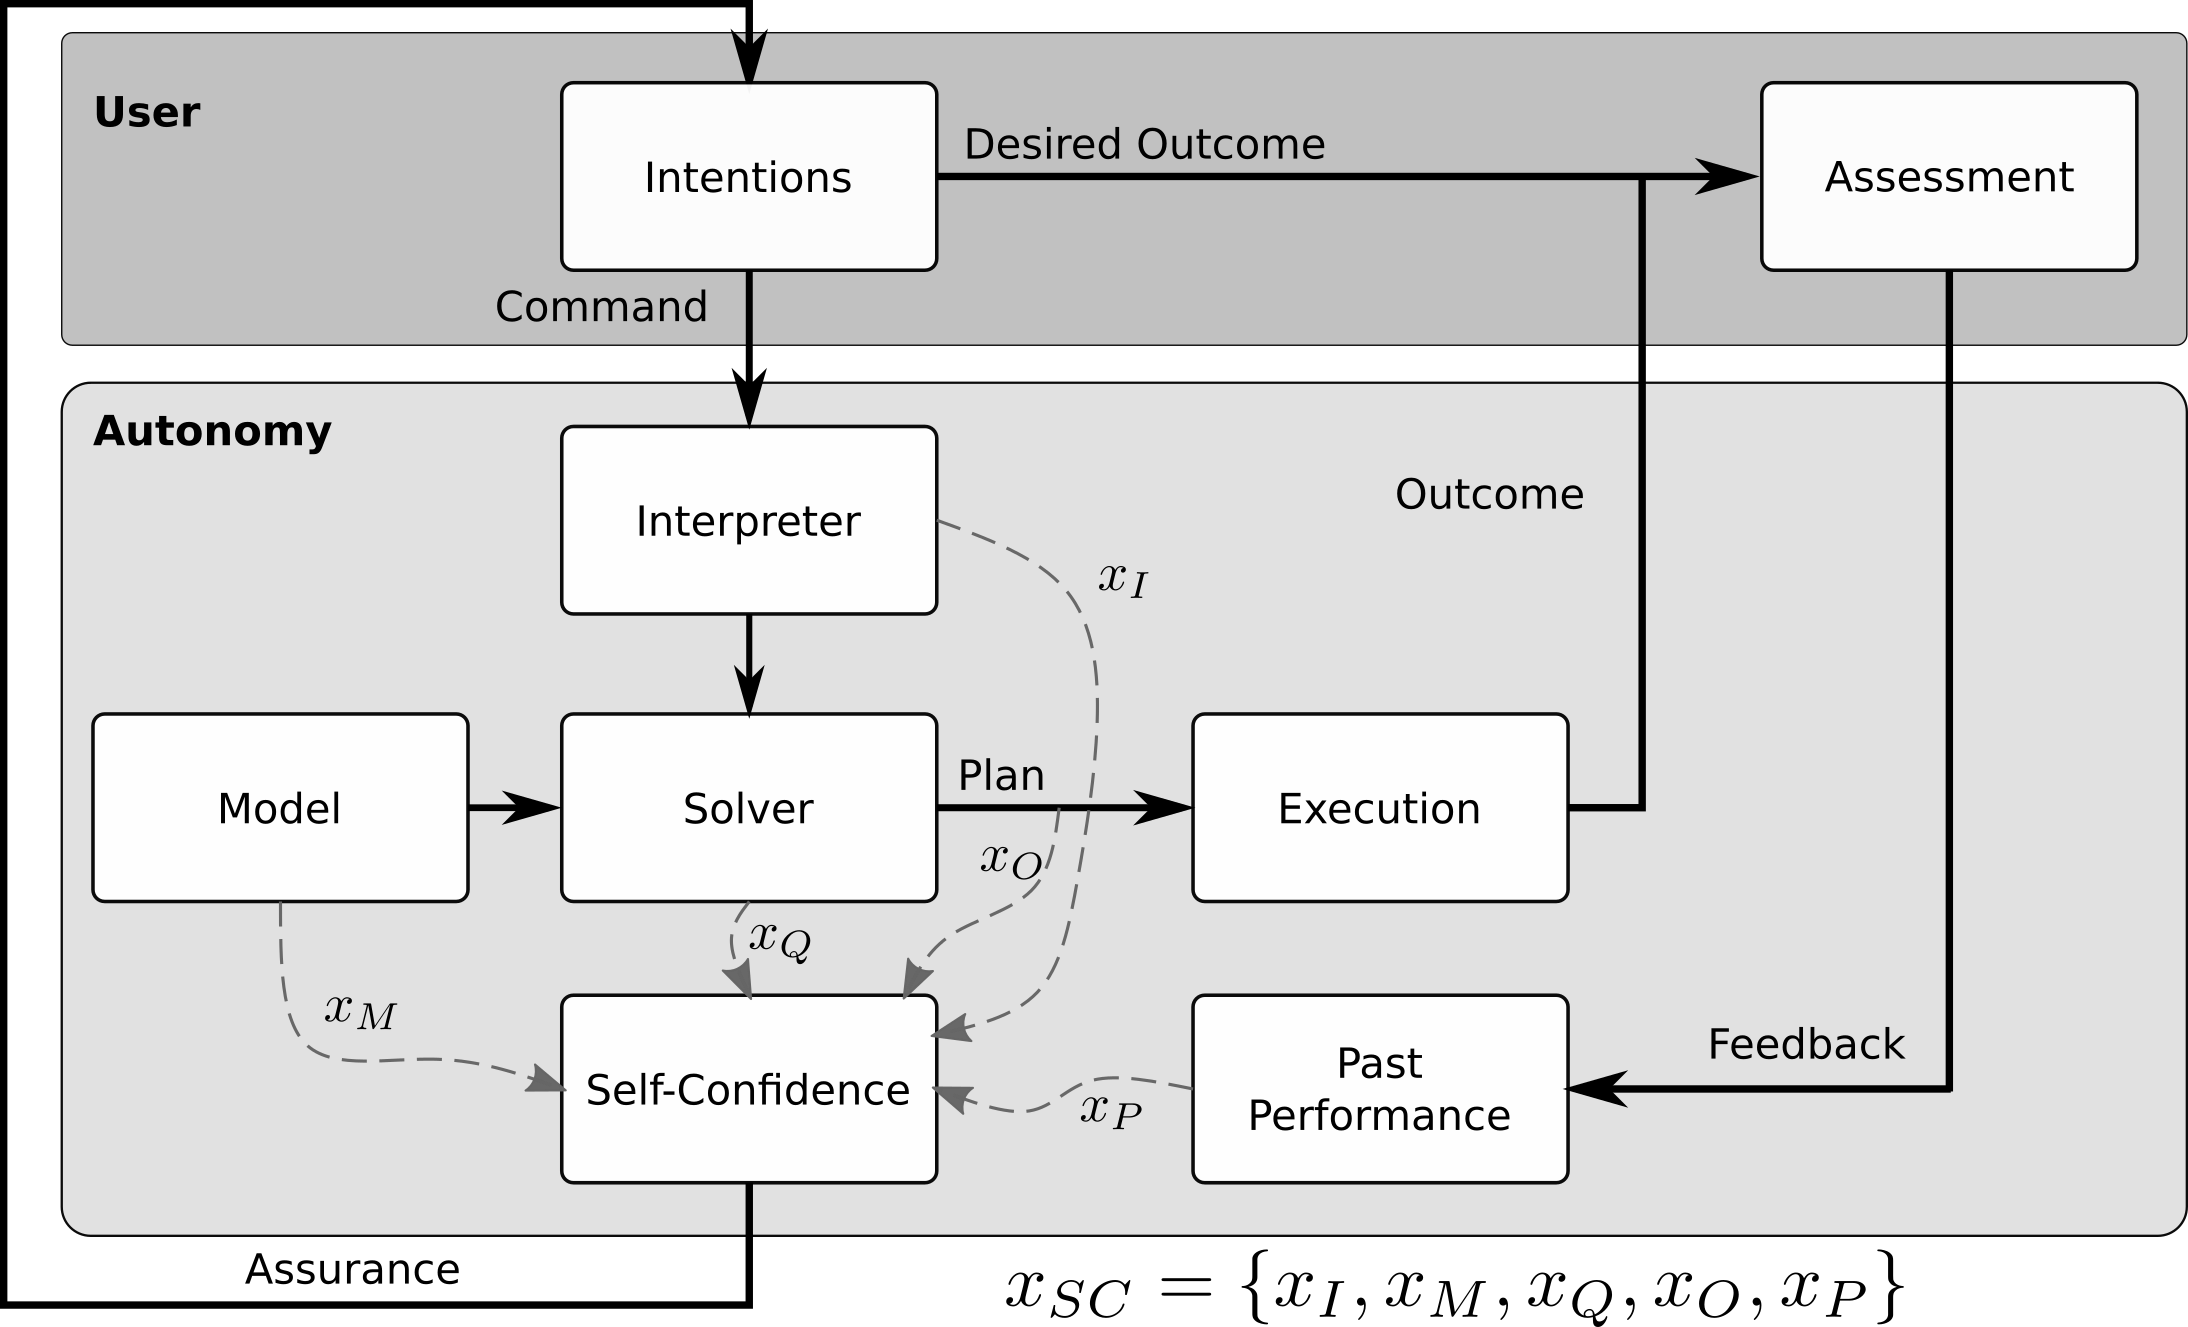
\includegraphics[width=0.95\linewidth]{Figures/FaMSeC.png}
        \caption{Factorized Machine Self-Confidence (FaMSeC)}
        \label{fig:famsec}
    \end{figure}
    
    \begin{figure}[tb]
        \centering
        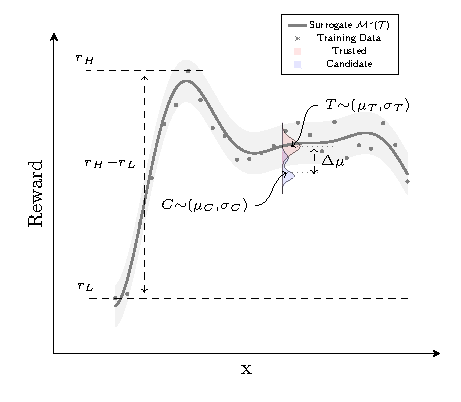
\includegraphics[width=0.9\linewidth]{Figures/sq_v2_fig}
        \caption{Figure that graphically depicts the key values involved in calculating \xQ. Here $x$ represents a `parameter of interest' of task \task. \nisar{get rid of excess whitespace around figure} }
        \label{fig:sq_v2}
    \end{figure}

   \nisar{move parts of this to Sect. 2, and add in some bits from process based eval from proposal, e.g. based on how expert would evaluate where/when approximations are expected to break down...} Several definitions of machine self-confidence have been proposed in recent works. Much of this work is reviewed in \cite{Israelsen2017-ym}, where self-confidence is identified as an explicit assurance in a human-autonomy trust relationship. According to \cite{Sweet2016-tz} the four views on self-confidence are the \textit{anthropomorphic view}, the \textit{uncertainty view}, the \textit{experiential view}, and the \textit{stability view}. The anthropomorphic view defines self-confidence to be similar to how humans express self-confidence, while the experiential view expresses self-confidence based on past experience. The uncertainty view simply defines self-confidence to be the probability of success or failure, and the stability view defines self-confidence to be the sensitivity of the probability of success to uncertainty. All of these views seem to reflect different parts of a more general concept: understanding an autonomy's ability to do a specific task. This leads to our definition of self-confidence: \textbf{An agent's perceived ability to achieve assigned goals (within a defined region of autonomous behavior) after accounting for (1) uncertainties in its knowledge of the world, (2) uncertainties of its own state, and (3) uncertainties about its reasoning process and execution abilities.}

    ...\nisar{edit:} The formal calculation of self-confidence we use is from \cite{Aitken2016-cv}, wherein five factors that compose self confidence are defined. Figure \ref{fig:famsec} highlights at what point in a autonomous system's logic each of the factors originate. They are: \nisar{can add some more detail from proposals...}

        \begin{itemize}
            \item [\xP{}:] \textbf{Past Performance}---how well has autonomy done in similar circumstances?
            \item [\xI{}:] \textbf{Command Interpretation}---are autonomy and user `on the same page'?
            \item [\xM{}:] \textbf{Model Validity}---How well does autonomy's model reflect reality?
            \item [\xO{}:] \textbf{Predicted Outcome Assessment}---How favorable is the distribution of predicted outcomes?
            \item [\xQ{}:] \textbf{Solver Quality}---How well can the solver use the model to generate policies/plans?
        \end{itemize}

    Self-confidence \xSC{} is a composite assurance that stems from some combination of these five factors. \xP{} has been previously defined in \cite{Aitken2016-cv}, but has not yet been evaluated as an effective assurance as per the guidelines laid out in the work on assurances. Herein \xQ{} is investigated. \nisar{edit...note that we are notionally using -1 to 1 range as a notional example here...do we later shift this range to 0 to 2 for \xQ?? (maybe note this here...or just change in table example below -- and/or maybe use this to underscore fact that ranges can be set arbitrarily and depending on context, e.g. see Hutchins paper...don't want to get too hung up on this...) }

\subsection{VIP Escort Example Revisited}
\nisar{TODO: talk about possible stochastic motion planning solvers (could be MDP family or others...) and discuss/move in table with example boundary conditions -- BE MINDFUL OF RANGE VALUES AS PER NOTE ABOVE...transition to talking about computation: start with pointing to Matt's thesis work for outcome assessment with brief mention of UPM/LPM...then transition to next section on how to compute solver quality}

\begin{figure}[tbp]
    \centering
    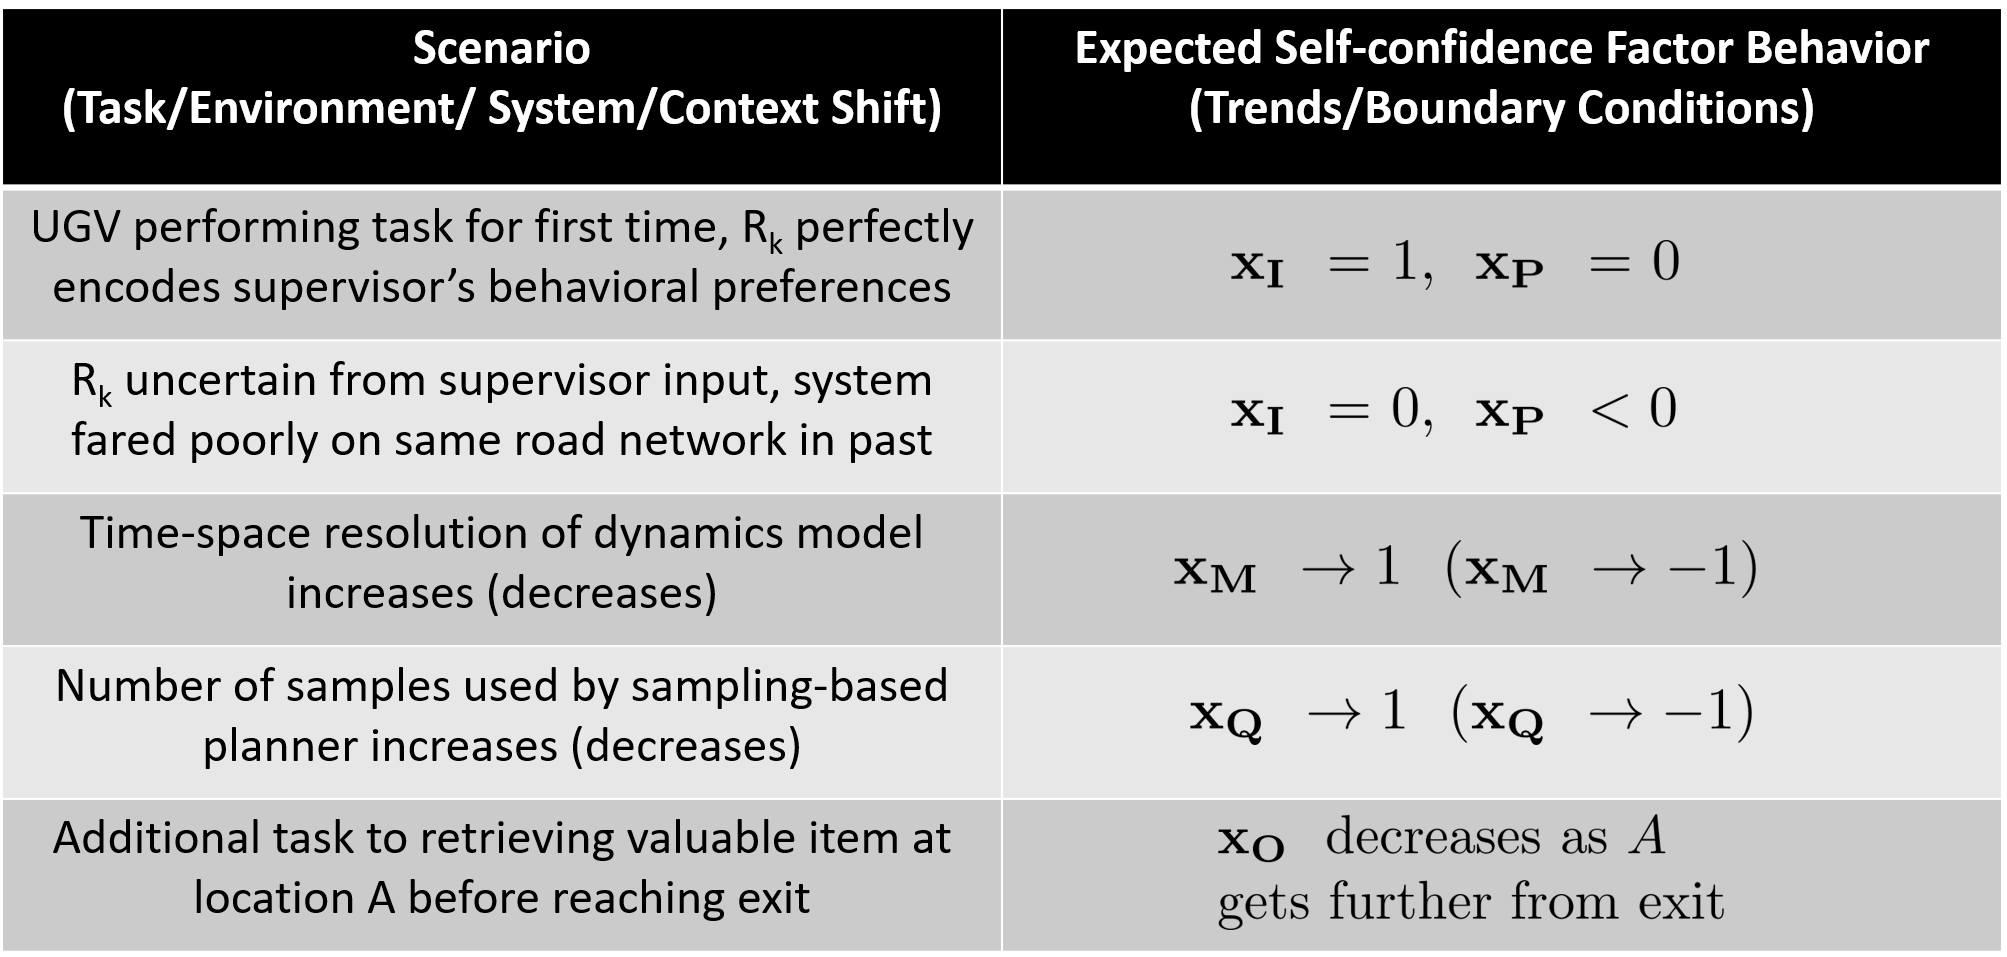
\includegraphics[width=0.95\linewidth]{Figures/scTrendsBoundaryExample.png}
    \caption{Notional \famsec behaviors for VIP Escort problem with a hypothetical stochastic planner.}
    \label{fig:roadnet}
\end{figure}

\begin{figure}[tbp]
    \centering
    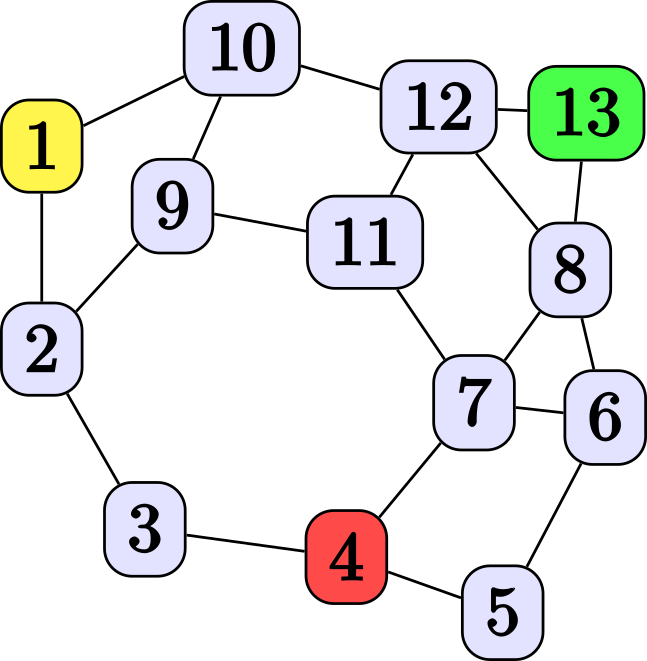
\includegraphics[width=0.4\linewidth]{Figures/original_roadnet.png}
    \caption{Diagram of the `Road Network' layout. Node 1 (yellow) is the start location of the UGV. Node 4 (red) is the start location of the pursuer vehicle. Node 13 (green) is the exit node. \nisar{MOVE TO RESULTS SECTION -- makes more sense to put this side by side the more complicated network to concretely show the change in \task... }}
    \label{fig:roadnet}
\end{figure}

\subsection{Solver Quality (\xQ)} \label{sec:SQ}
    The main aim of \xQ{} is to indicate how a solver \solve{} will perform on a given (possibly un-encountered) task \task{}. Formally, the desiderata are:

    \begin{enumerate}[label=\textbf{D\arabic*}]
        \item reflect competence of solver \solve{} for task \task{} \label{itm:d1}
        \item enable comparison across solver classes \label{itm:d2}
        \item extend to unseen tasks \label{itm:d3}
    \end{enumerate}
    
    Evaluating the `quality' of something implies some kind of comparison is taking place. In this setting the desired comparison is between a `candidate solver' \solve{} and some reference solver. Ideally, the candidate solver could be compared to the exact solution, but there are three main challenges:

    \begin{enumerate}[label=\textbf{C\arabic*}]
        \item It is unclear how policies should be compared \label{itm:l1}
        \item Exact solutions to most practical problems are infeasible due to large state-spaces \label{itm:l2}
        \item Even if \ref{itm:l2} weren't an issue, it is generally impossible to evaluate the performance of any solver on \emph{all} possible problems \label{itm:l3} of a given class
    \end{enumerate}

    \subsubsection{Addressing \ref{itm:l1}} \label{sec:compare_policies}
        Solvers of all classes are similar in that they operate on a specified problem, in order to produce a policy $\pi$ that is a mapping from states to actions. A few possibilities for comparing policies include:
    
        \begin{enumerate}
            \item Compare utilities at each state \label{itm:i1}
            \begin{itemize}
                \item Merits: Evaluates whether states are assigned equal utility across solvers. Theoretically state utilities should be independent of the solver. Addresses \ref{itm:d1}
                \item Demerits: Does not apply to solvers that represent different amounts of the state-action space (i.e. exact versus approximate solvers), or to solvers that may represent the state-action space differently (i.e. meta-solvers). This approach does not satisfy \ref{itm:d2}.
            \end{itemize} 
            \item Compare `coverage' of the policy (here coverage refers to the proportion of the state space considered by the solver) \label{itm:i2}
            \begin{itemize}
                \item Merits: Evaluates how `thorough' the policy is, in concert with \ref{itm:i1} could address \ref{itm:d1}
                \item Demerits: Does not meet \ref{itm:d2} because not all policies will have the same coverage by design. Also high coverage does not imply a `good' solution
            \end{itemize}
            \item Compare the reward distribution of given policies \label{itm:i3}
            \begin{itemize}
                \item Merits: Meets \ref{itm:d1}, also able to satisfy \ref{itm:d2} as reward distributions can be simulated from any policy
                \item Demerits: Expensive to calculate the reward distribution via many simulations
            \end{itemize}
        \end{enumerate}

        Of the possibilities listed above, item \ref{itm:i3} will be used because only it is able to satisfy \ref{itm:d1} and \ref{itm:d2}.

    \subsubsection{Addressing \ref{itm:l2}, and \ref{itm:l3}} \label{sec:practicality}
        In order to address \ref{itm:l2} a `trusted solver' \solvestar{} could be introduced as the reference to which the candidate solver \solve{} can be compared. This solver need not be exact (but could be). Ultimately, \solvestar{} is only required to be a reference of some kind; it may be optimal, or it may be abysmal. In fact given a space of all possible unseen tasks of class $\text{some task class notation}$, \solvestar{} will likely be abysmal for some of them.

        Still, according to \ref{itm:l3}, it is impractical, or impossible, to find an exact solution for all tasks $\text{task class notation}$. Literature on `Empirical Hardness Models' (EHMs) lends some direction for confronting this challenge. In their work \cite{Leyton-Brown2009-yr,Hutter2009-og} introduced EHMs in order to predict the empirical runtime performance of an algorithm on a problem with given features \brett{add some more detail about the approach, I think they used SAT*}. Applying similar logic in this domain, it should be possible to learn a surrogate model \surrogate{} that predicts the reward distribution \rwdstarapprox{} of the trusted solver \solvestar{} for a given task \task. In this way it is possible to estimate the performance of \solvestar{} on problems to which it has never been applied.
